\documentclass[10pt]{report}

\usepackage{talk}
\usepackage[export]{adjustbox}

\newcommand{\draw}[2]{#1^{(#2)}}
\newcommand{\displayfrac}[2]{{\displaystyle \frac{\displaystyle #1}{\displaystyle #2}}}
\newcommand{\simvar}[1]{#1^{\textrm{sim}}}
\newcommand{\simdraw}[2]{#1^{\textrm{sim}(#2)}}

\begin{document}
\sf%
\mbox{ }
\\[12pt]
\spc{\LARGE\bfseries \myemph{What do we need from a PPL}}
\\[8pt]
\spc{\LARGE\bfseries \myemph{to support Bayesian workflow?}}
\\[36pt]
\noindent
\spc{\Large\bfseries \myemph{Bob Carpenter}}
\\[4pt]
\spc{\large Center for Computational Mathematics}
\\[2pt]
\spc{\large Flatiron Institute}
\vfill
\noindent
\spc{\small October 2021} \hfill
{\small \myemph{ProbProg 2021}}

% \mypart{}{Motivation}

\pagestyle{plain}

\sld{What is Bayesian workflow?}
\begin{itemize}
\item Bayesian workflow involves
  \begin{subitemize}
  \item developing models,
  \item fitting models to data,
  \item validating computation,
  \item evaluating and using models,
  \item modifying models,
  \item addressing computational issues, and
  \item comparing models.
    \vfill
  \end{subitemize}
  \item \footnotesize Gelman, Vehtari, Simpson, Margossian, Carpenter, 
    Yao, Kennedy, Gabry, Bürkner, and Modrák. 2020. \myemph{Bayesian workflow}. 
    \textit{arXiv} 2011.01808.
  \item Book draft: \url{https://github.com/jgabry/bayes-workflow-book}
\end{itemize}

\sld{Bayesian model}
\begin{itemize}
\item $y$ is \myemph{observed data}, $\theta$ are \myemph{unknown parameters}
\begin{subitemize}
\item suppress unmodeled predictors/features $x$
\end{subitemize}
\item \myemph{prior} $p(\theta)$
\item \myemph{sampling} $p(y \mid \theta)$
  \begin{subitemize}
    \item likelihood $\mathcal{L}(\theta) = p(y \mid \theta)$ for fixed $y$
  \end{subitemize}
\item \myemph{joint} $p(y, \theta)$
\item \myemph{posterior} $p(\theta \mid y)$
\end{itemize}

\sld{Bayesian inference is expectation}
\begin{itemize}
\item \myemph{parameter estimate} \ $\hat{\theta} = \mathbb{E}[\theta \mid y]$
\item \myemph{event probability} \ $\textrm{Pr}[C] = \mathbb{E}[I_C(\theta) \mid
  y]$
\item \myemph{posterior predictive} \ $p(\tilde{y} \mid y) =
  \mathbb{E}[p(\tilde{y} \mid \theta) \mid y]$
\end{itemize}

\sld{Expectations via Monte Carlo}
\begin{itemize}
  \item calculate \myemph{asymptotically exact} expectations by averaging
\begin{eqnarray*}
  \mathbb{E}[f(\theta) \mid y]
  & = & \textstyle \int_{\Theta} f(\theta) \cdot p(\theta \mid y) \,
        \textrm{d}\theta
        \\[4pt]
  & = & \textstyle \lim_{M \rightarrow \infty} \frac{1}{M} \sum_{m = 1}^M
        f(\draw{\theta}{m})
        \\[4pt]
  & \approx & \textstyle \frac{1}{M} \sum_{m = 1}^M (\draw{\theta}{m}),
\end{eqnarray*}
\item MCMC \myemph{central limit theorem} says that if draws
\[
  \draw{\theta}{1}, \ldots, \draw{\theta}{M} \sim p(\theta \mid y)
\]
have \myemph{effective sample size} $M_{\textrm{eff}}$, then
\[
\textrm{standard error (of estimate)}
  = \displayfrac{\textrm{posterior standard deviation}}
                {\sqrt{M}_{\textrm{eff}}} 
\]
\end{itemize}

\sld{Probabilistic programs typically $\ldots$}
\begin{itemize}
\item code Bayesian joint densities
\item support sampling from the posterior to compute expectations
\begin{subitemize}
\item often with approximate variational posteriors
\item sometimes with acceleration like control variates
\end{subitemize}
\vfill
\item but it turns out that we
  \\
  \myemph{need more than posterior sampling for workflow}
\end{itemize}

\sld{Workflow flowchart}
\begin{center}
\vspace*{-6pt}
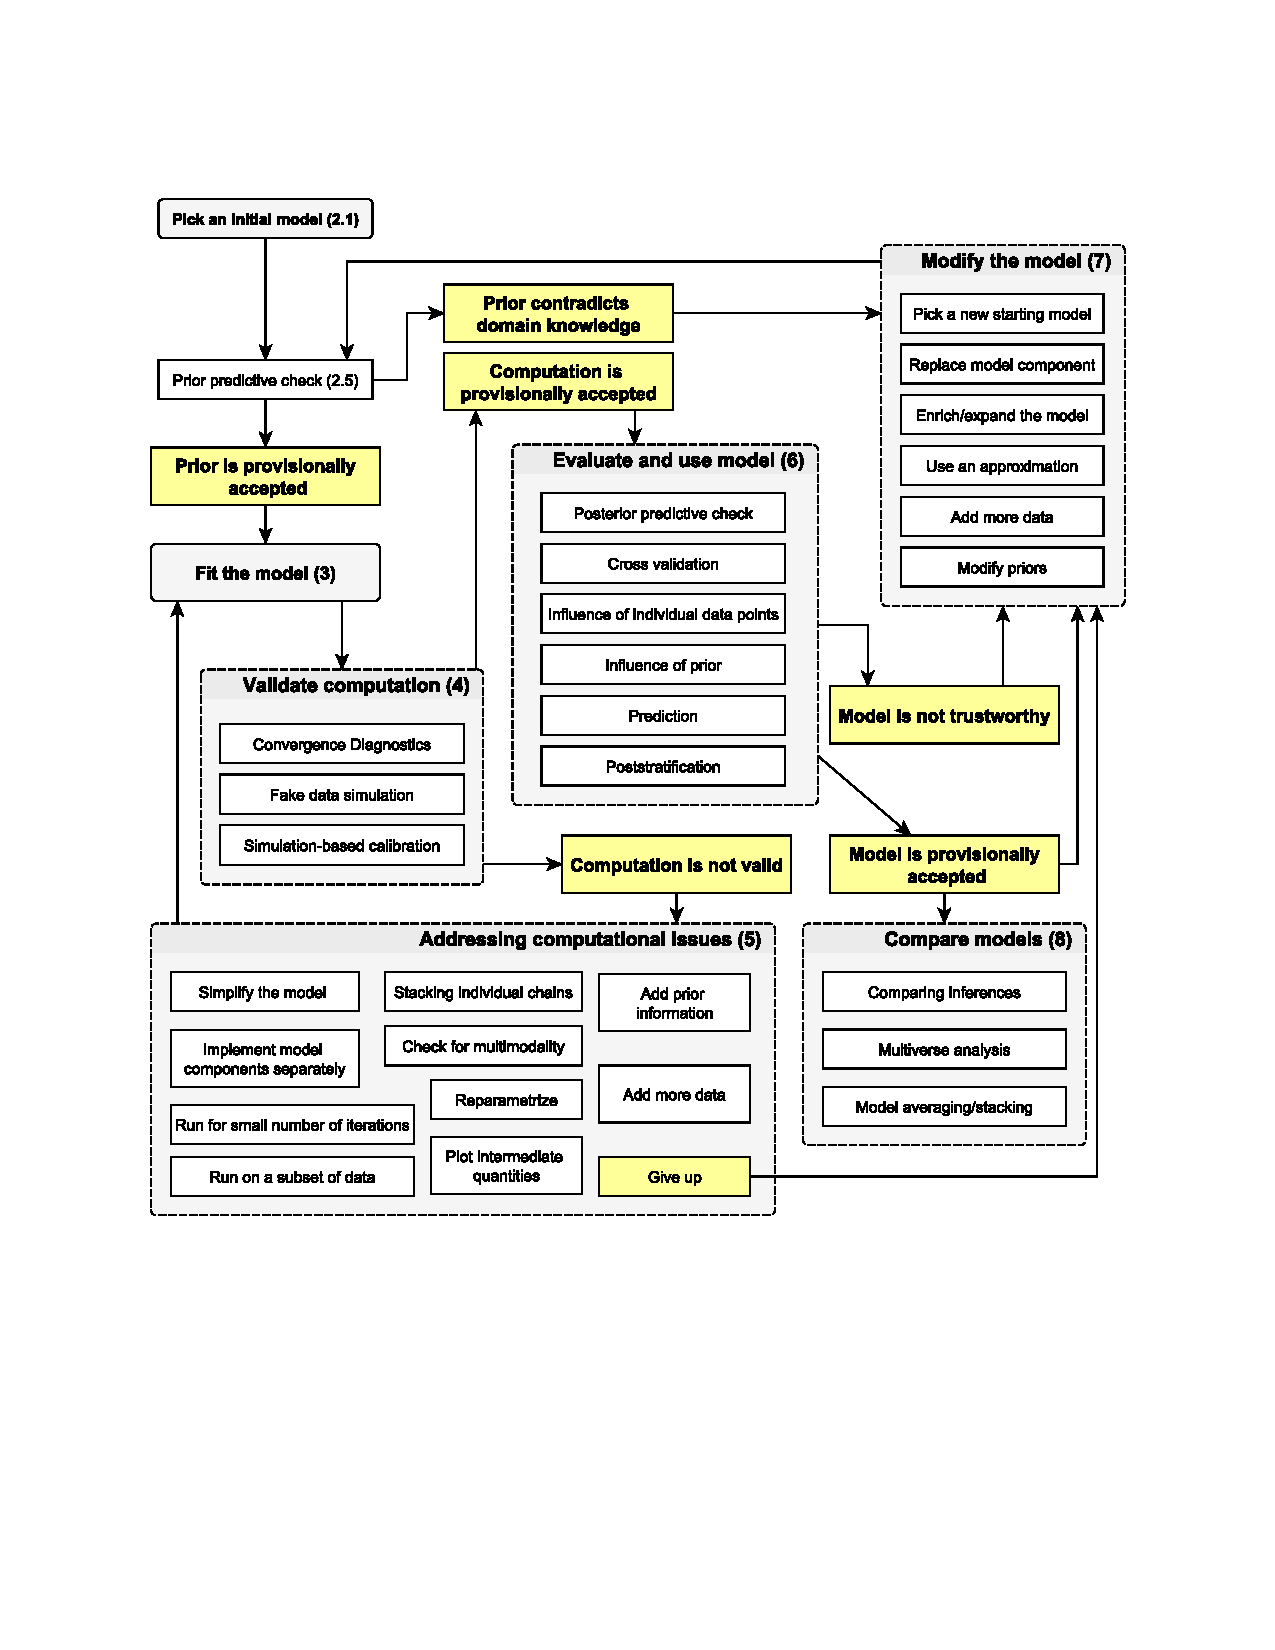
\includegraphics[height=0.9\textheight]{img/workflow-fig.pdf}
\end{center}

\sld{Prior predictive checks}
\begin{itemize}
\item prior predictive checks simulate data from the marginal
  \[
    \simvar{y} \sim p(y)
  \]
\item often by generating from prior and sampling distributions
  \[
    \simvar{\theta} \sim p(\theta)
    \qquad
    \simvar{y} \sim p(y \mid \simvar{\theta})
  \]
\item then we compare simulated data $\simvar{y}$ to observed $y$
  \vfill
  {\tiny Gabry, Simpson, Vehtari, Betancourt,
    Gelman. 2019. Visualization in Bayesian workflow. \textit{JRSS A}.}
\end{itemize}

\sld{Prior predictive example}

\begin{center}
\vspace*{-8pt}
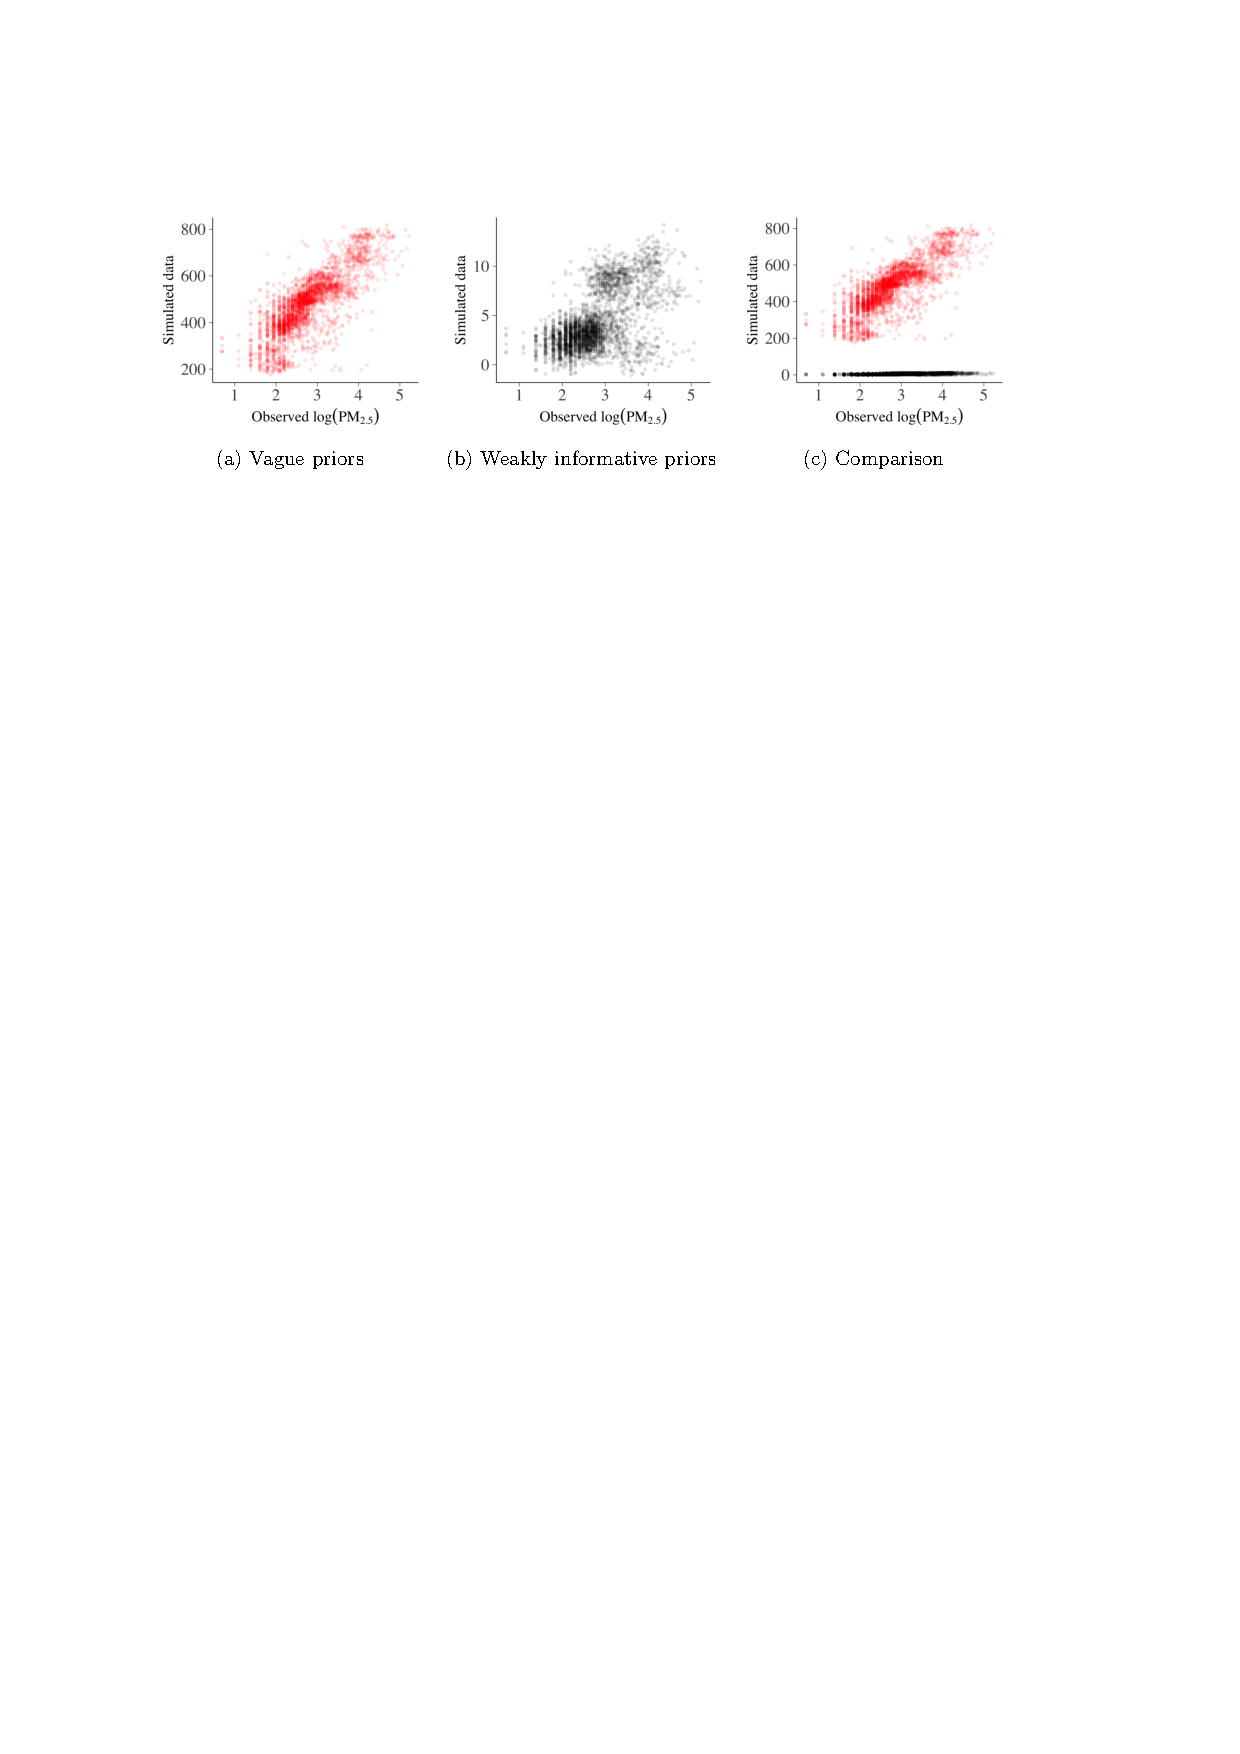
\includegraphics[width=0.9\textwidth]{img/prior-predictive-eg.pdf}
\end{center}
\vspace*{-10pt}
\begin{itemize}
\item \myemph{particulate matter pollution} model with prior on
  $\log(\textrm{PM}_{2.5})$
\item \myemph{vague prior} generates values as dense as neutron star
\item \myemph{weakly informative} prior controls scale
\item subtle with priors on \myemph{interacting parameters}
  \begin{subitemize}
  \item why we need a PPL!
  \end{subitemize}
\end{itemize}

\sld{How does Stan fare?}
\begin{itemize}
\item Stan model for \myemph{posterior inference}
\vspace*{-6pt}
{\footnotesize
\begin{verbatim}
  data { int<lower=0> N; int<lower=0, upper=1> y[N]; }
  parameters { real<lower=0, upper=1> theta; }
  model { theta ~ beta(2, 10);  y ~ binomial(theta); }
\end{verbatim}
}
\item Simulate $\simvar{\theta} \sim p(\theta)$ with $N = 0$, but
  can't simulate $y$
\item Stan model for \myemph{prior predictive checks}
\vspace*{-6pt}
{\footnotesize
\begin{verbatim}
  data { int N; }
  parameters { real<lower=0, upper=1> theta; }
  model { theta ~ beta(2, 10); }
  generated quantities { 
    int y[N] = bernoulli_rng(N, theta); }
\end{verbatim}
}
\end{itemize}

\sld{How do other PPLs fare?}
\begin{itemize}
\item \myemph{PyMC3} also declares data with \myemph{\texttt{observed=}}
\vspace*{-6pt}
{\footnotesize 
\begin{verbatim}
    y_obs = pm.Normal("y_obs", mu=X @ weights, 
                      sigma=noise, observed=y) 
\end{verbatim}
\vspace*{-8pt}
}
\item \myemph{ADMB} declares data in a \myemph{\texttt{DATA SECTION}}
\item \myemph{Pyro} uses effect handler \myemph{\texttt{condition()}} for data, e.g., 
\vspace*{-6pt}
{\footnotesize 
\begin{verbatim}
    poutine.condition(model, data={"z": 1.0})
\end{verbatim}
\vspace*{-8pt}
}
\item \myemph{Turing.jl} assigns data variables before
  just-in-time compilation; values may be specified
  \myemph{\texttt{missing}}
\item \myemph{BUGS} sets data at run time w.r.t.\ its neutral graphical model
\vspace*{-12pt}
{\footnotesize 
\begin{verbatim}
  theta ~ dbeta(2, 10); for (n in 1:N) y[n] ~ dbern(theta); 
\end{verbatim}}
\end{itemize}


\sld{Simulation-based Calibration}
\begin{itemize}
\item to \myemph{validate inference} w.r.t.\ well-specified data
  \begin{subitemize}
    \item approximate inference like VI will fail
    \end{subitemize}
  \item draw $\simvar{\theta} \sim p(\theta)$ from the prior
  \item draw $\simvar{y} \sim p(y \mid \simvar{\theta})$ from the
    sampling distribution
  \item draw $\draw{\theta}{1}, \ldots, \draw{\theta}{M} \sim p(\theta
    \mid \simvar{y})$ from algorithm to test
  \item because $(\simvar{y}, \simvar{\theta}) \sim p(y, \theta)$ and
    $(\simvar{y}, \draw{\theta}{m}) \sim p(y, \theta)$,
    $\simvar{\theta}$ should have uniform rank among the
    $\draw{\theta}{m}$
    \vfill
    {\tiny $\bullet$\ Cook,  Gelman, Rubin.
      2006. Validation of software for Bayesian models using posterior
      quantiles. \textit{JCGS}.
      \\
      $\bullet$\ Talts, Betancourt, Simpson, Vehtari, Gelman. 2018. Validating Bayesian inference algorithms with simulation-based calibration. \textit{arXiv}}
\end{itemize}

\sld{SBC diagnoses}
\begin{itemize}
  \item 
    \myemph{over-dispersed}: \hfill
    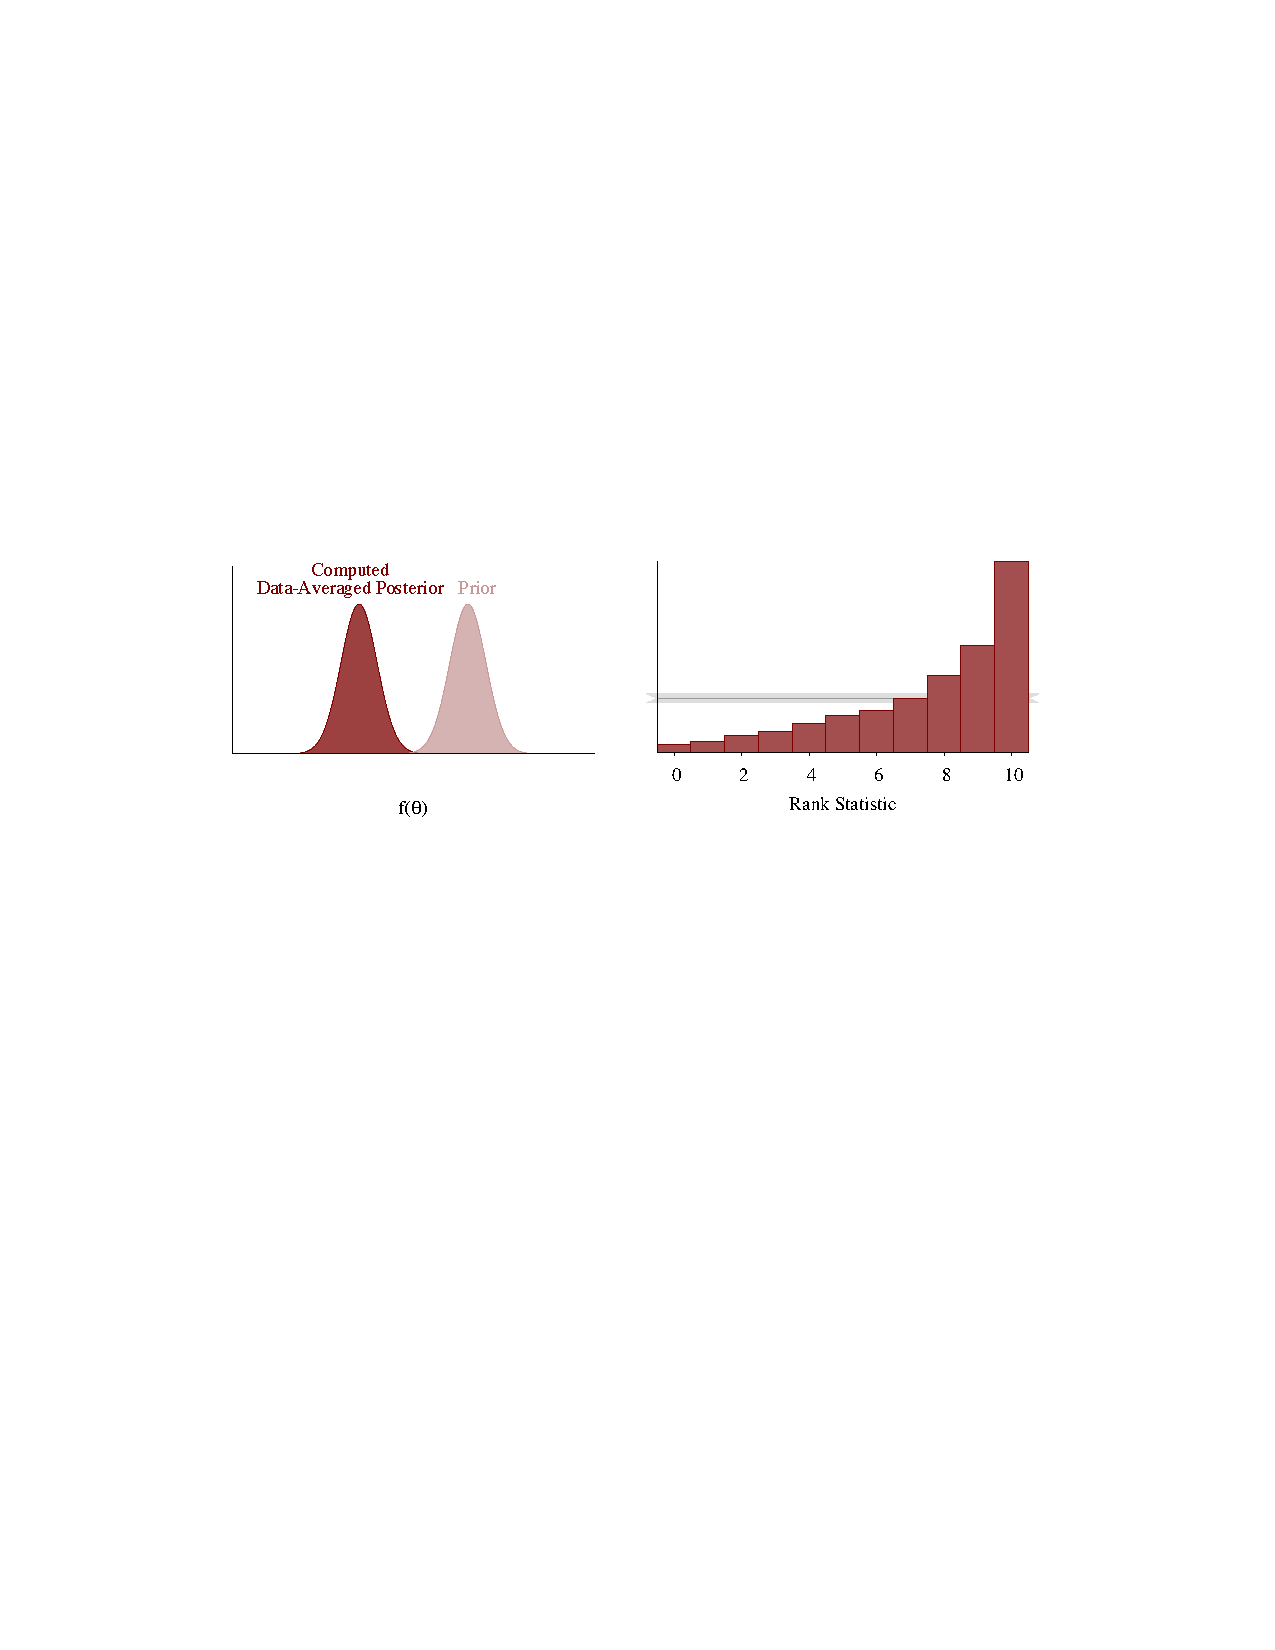
\includegraphics[valign=c,width=0.5\textwidth]{img/sbc-over.pdf}
  \item 
    \myemph{under-dispersed}: \hfill
    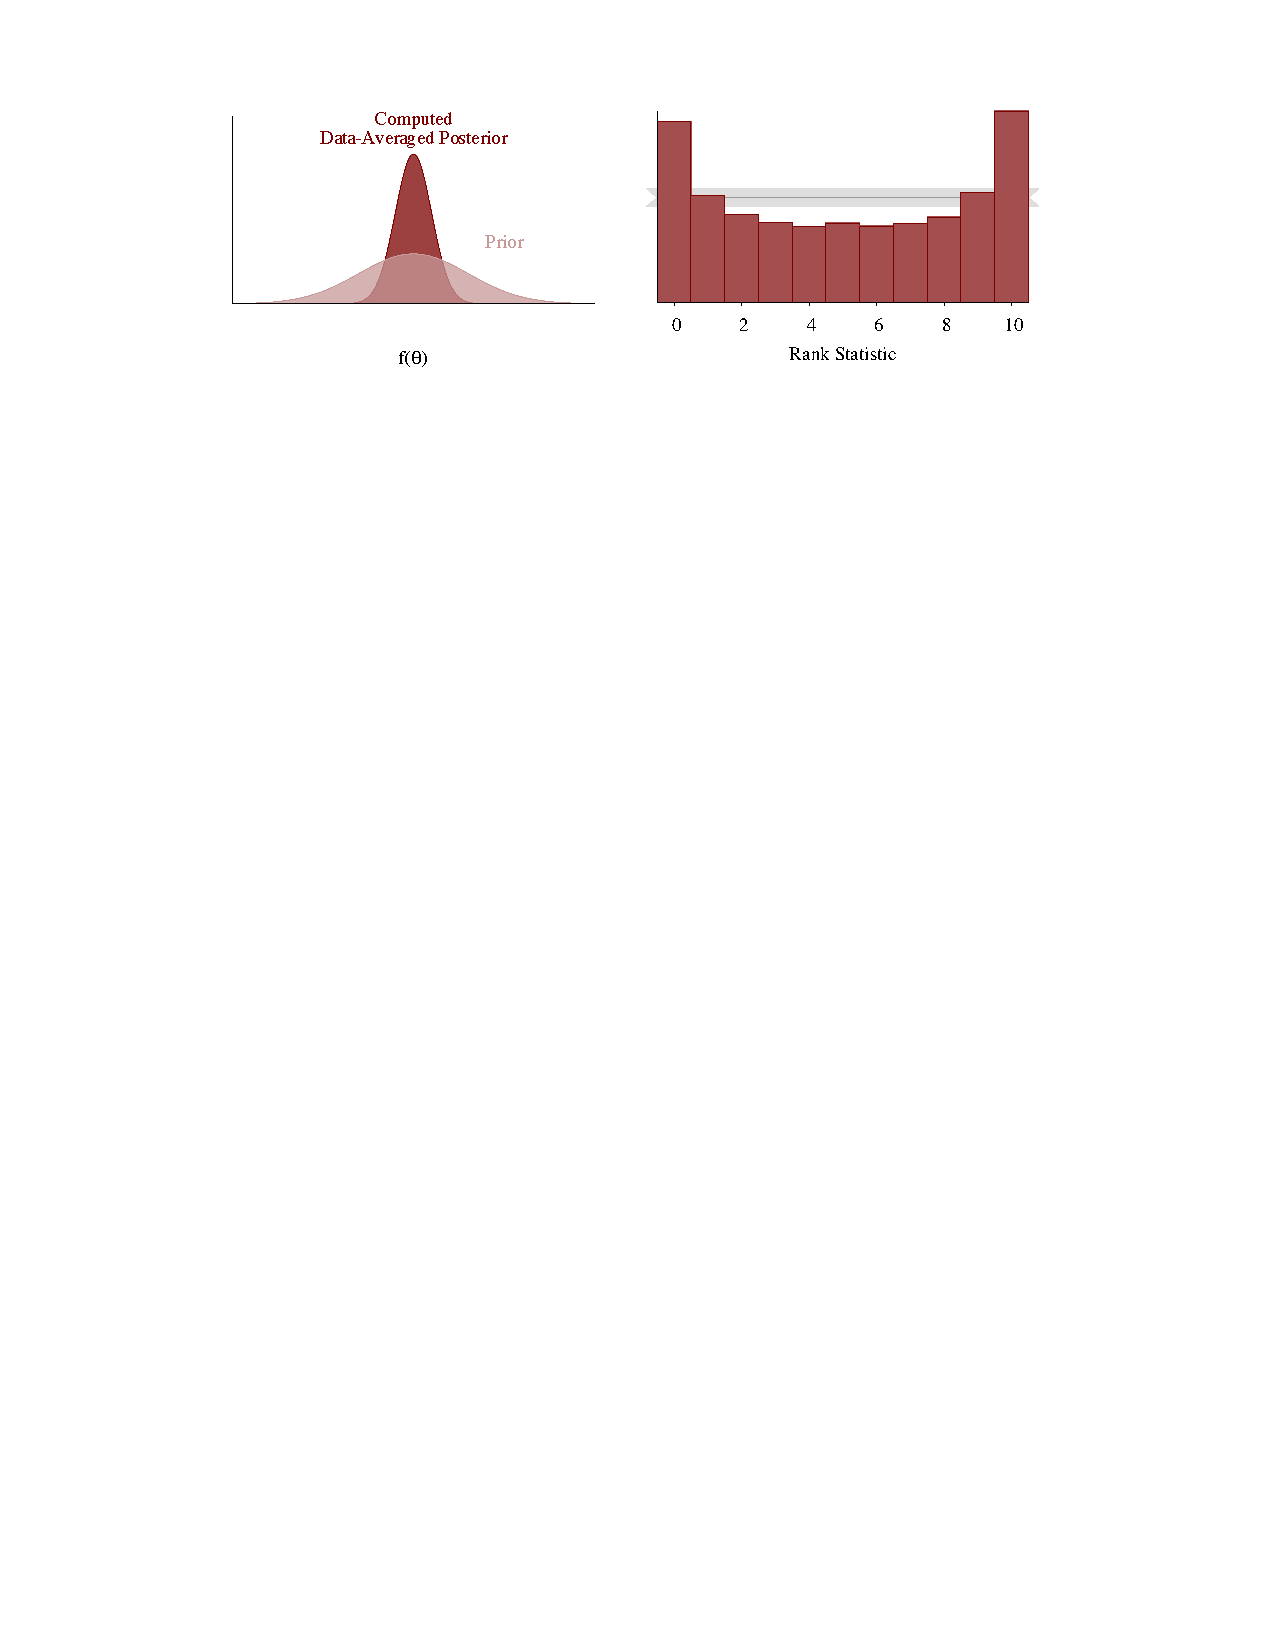
\includegraphics[valign=c,width=0.5\textwidth]{img/sbc-under.pdf}
  \item 
    \myemph{skewed}: \hfill
    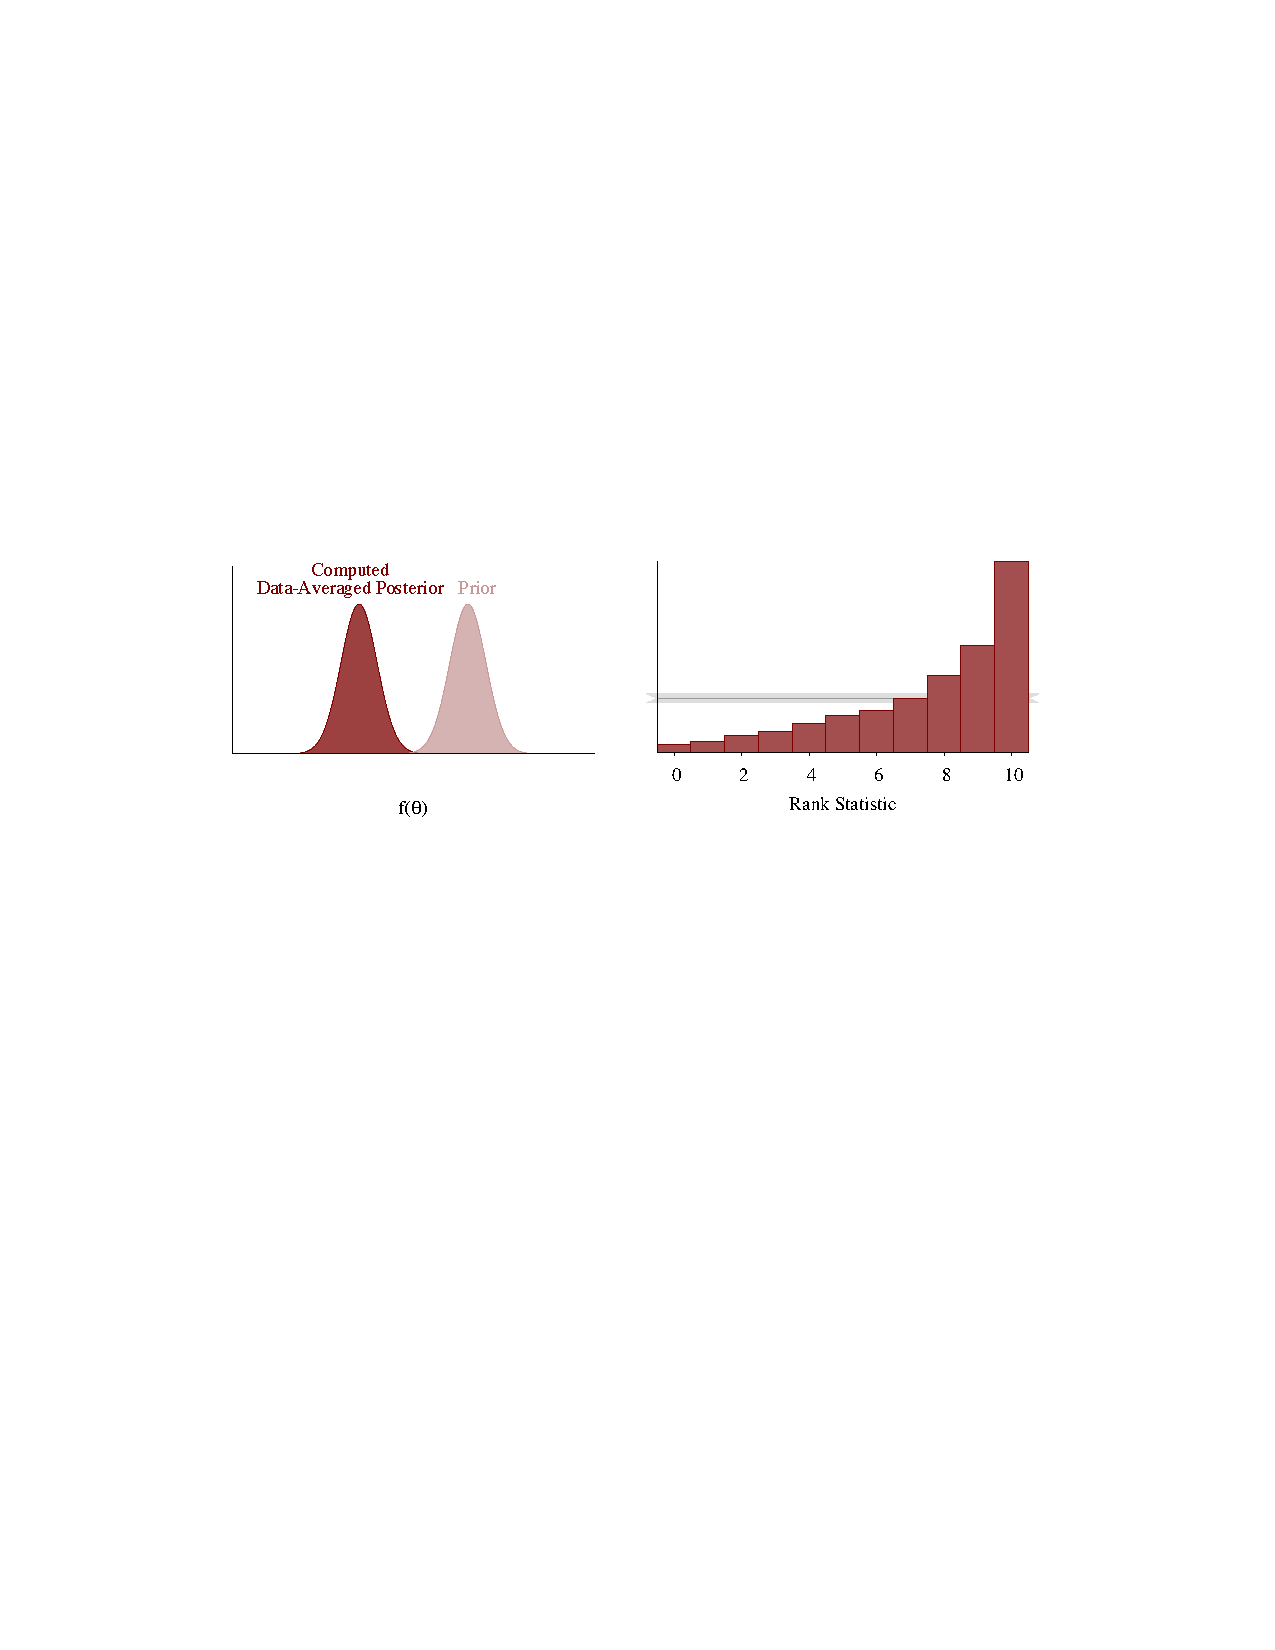
\includegraphics[valign=c,width=0.5\textwidth]{img/sbc-skew.pdf}
\end{itemize}



\sld{How do PPLs fare on SBC?}

\begin{itemize}
\item simulation-based calibration requires simulating from prior and
  sampling distribution
\item presents same problem with data specification as prior
  predictive checks
\end{itemize}

\sld{Posterior predictive checks}
\begin{itemize}
\item Simulate new data from posterior for draws $m \in 1{:}M$,
  \begin{eqnarray*}
    \draw{\theta}{m} & \sim & p(\theta \mid y)
    \\
    \simdraw{y}{m} & \sim & p(y \mid \draw{\theta}{m})
  \end{eqnarray*}
\item Compare statistics $s(y)$ on observed data to those
  of posterior simulations $s(\simdraw{y}{m})$, e.g.,
  \begin{subitemize}
  \item $s()$ can be anything, e.g., mean, max, sd, quantiles, ranks,
    skew, etc.
  \end{subitemize}
\item Plot, or compute two-sided posterior $p$-values to automate,
  \[
    p\textrm{-value} = \min(\begin{array}[t]{l}
                              \textrm{Pr}[s(y) < s(\simvar{y})],
                              \\[4pt]
                              1 - \textrm{Pr}[s(y) < s(\simvar{y})] \ )
                              \end{array}
  \]
\end{itemize}

\sld{Posterior predictive example}
\begin{center}
\vspace*{-10pt}
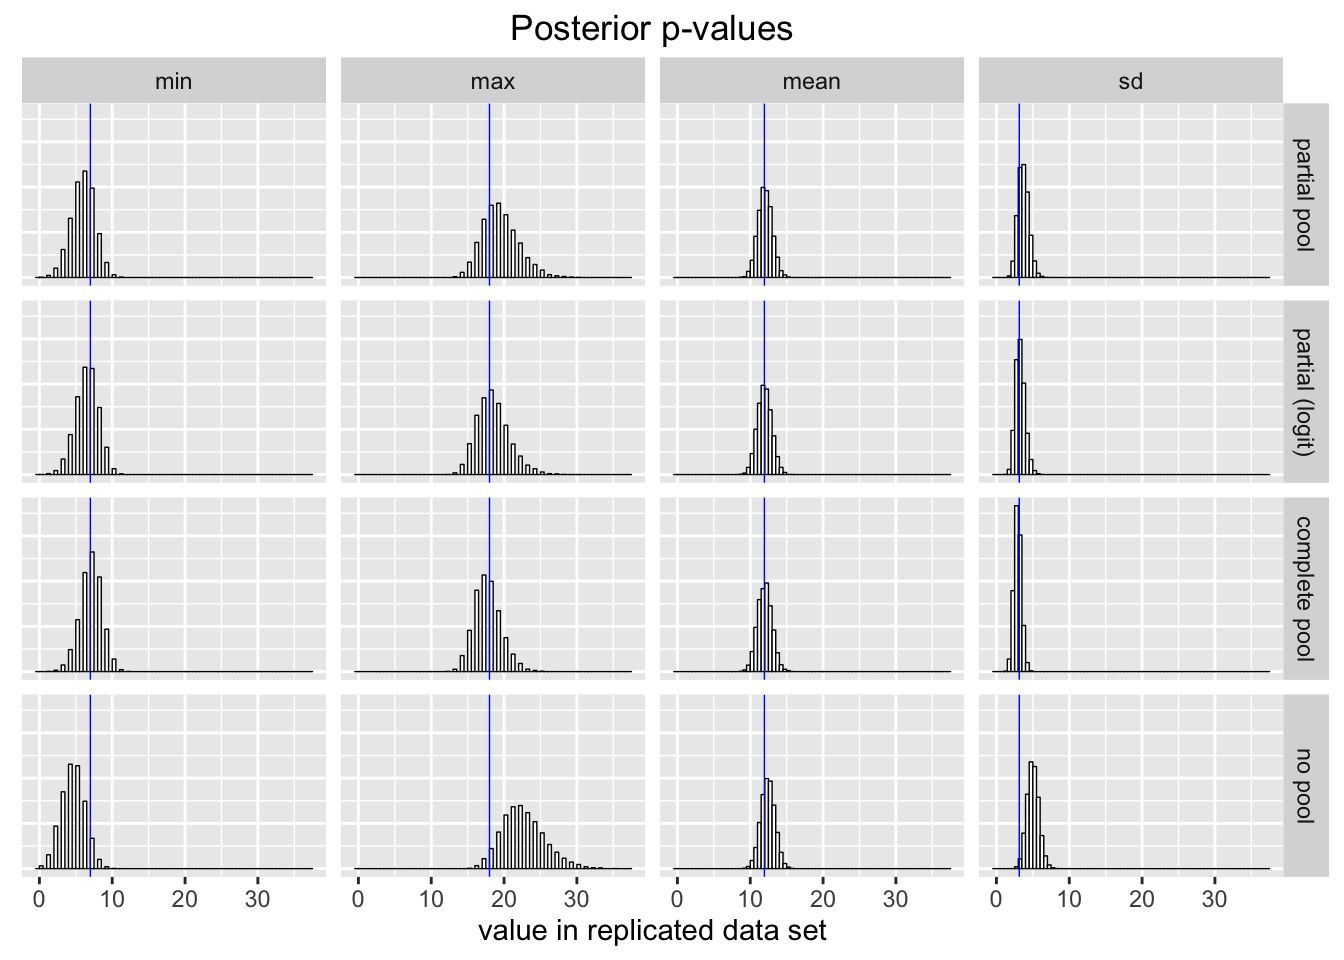
\includegraphics[width=0.6\textwidth]{img/ppc-binary-trials.png}
\vspace*{-10pt}
\end{center}
\begin{itemize}
\item model of repeated binary trials (baseball batting avg.)
  \begin{subitemize}
    \item vertical line is $s(y)$, histogram is $s(\simdraw{y}{m})$
    \item max() and sd() statistics ``reject'' the no-pooling model
  \end{subitemize}
\end{itemize}

\sld{PPL support for PPCs}
\begin{itemize}
\item requires extracting posterior draws and simulating data from
  them
\item still the same problem of flexibly specifying data
  vs.\ parameters (i.e., knowns vs.\ unknowns)
\end{itemize}

\sld{Cross-validation}
\begin{itemize}
\item divide data into train/test split (say $y$ and $\widetilde{y}$)
\item fit model on training set
\item evaluate predictive log density on test set,
  \begin{eqnarray*}
    \log p(\tilde{y} \mid y)
    & \approx & \log \frac{1}{M} \sum_{m=1}^M p(\tilde{y} \mid \simdraw{\theta}{m})
    \\[4pt]
    & = & \textrm{log-sum-exp}_{m=1}^M \, \log p(\tilde{y} \mid
          \simdraw{\theta}{m})
          - \log(M)
  \end{eqnarray*}
\end{itemize}

\sld{PPL support for X-val}
\begin{itemize}
\item this is trickier as now we have to fit with one data set $y$
  and evaluate with another
\item \myemph{BUGS} almost succeeds
\vspace*{-8pt}
{\footnotesize 
\begin{verbatim}
  for (n in 1:N) y[n] ~ dnorm(alpha + x[n] * beta, tau)
  tau ~ gamma(1, 1);  alpha ~ normal(0, 2);  beta ~ normal(0, 2)
\end{verbatim}
\vspace*{-8pt}}
by letting $y = y^{\textrm{train}}, y^{\textrm{test}}$ be partially
missing
\begin{subitemize}
  \item but doesn't let you retrieve the log density values for $y^{\textrm{test}}$
\item this also seamlessly handles missing data (that's modeled)
\end{subitemize}
\item \myemph{Turing.jl} allows the same thing (values?)
\item other PPLs require additional sampling statements for the test data
\end{itemize}  

\sld{Stan for X-val}
\begin{itemize}
\item Stan codes \myemph{leave-one-out X-val} by specifying test point
\vspace*{-6pt}
{\footnotesize 
\begin{verbatim}
data { 
  int N; int[N] y;  int nt;
}
parameters { 
  real mu; real<lower=0> sigma;
}
model { 
  append_row(y[:nt-1], y[nt+1:]) ~ normal(mu, sigma);
  mu ~ normal(0, 1);  sigma ~ lognormal(0, 1);
}
generated quantities {
  real lp = normal_lpdf(y[nt] | mu, sigma);
}
\end{verbatim}
  \vspace*{-8pt}}
\item but it's a \myemph{totally different model}
\end{itemize}

\sld{Sensitivity analysis}
\begin{itemize}
\item we'd like to understand how changes in our model affect
  posterior inference
\item e.g., vary priors and see how posterior expectations changes
\item all PPLs let you evaluate alternative constants easily
\item derivative-based sensitivity w.r.t.\ const. $c$ is trickier
  \[
    \frac{\partial}{\partial c} \mathbb{E}[f(\theta) \mid y, c]
  \]
  Ryan Giordano modified Stan's C++ to compute this for his (Berkeley)
  Ph.D. thesis, but it's not exposed
\end{itemize}  

\sld{Sensitivity example}
\begin{center}
\vspace*{-10pt}
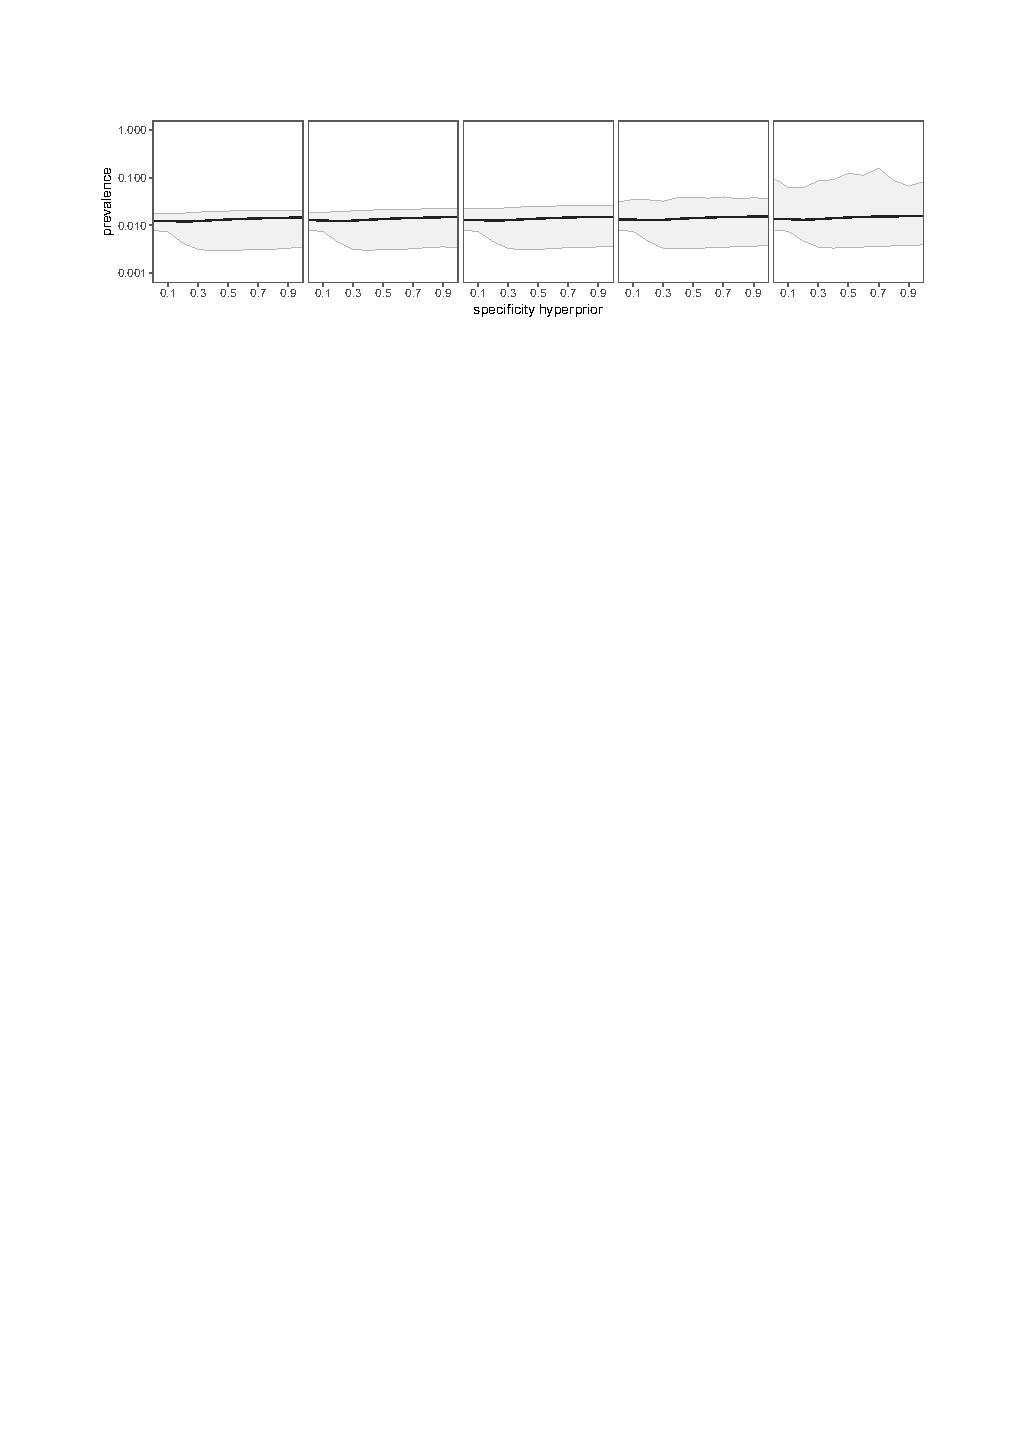
\includegraphics[width=0.9\textwidth]{img/covid-sensitivity.pdf}
\vspace*{-10pt}
\end{center}
\begin{itemize}
\item Estimated Covid seroprevalence as a function of
  \begin{subitemize}
  \item the hyperprior for specificity ($x$-axis)
  \item the hyperprior for sensitivity (facets with values from left-to-right
    0.01, 0.25, 0.5, 0.75, 1.0)
  \end{subitemize}
\vfill
{\tiny
Gelman, Carpenter. 2020. Bayesian analysis of tests with unknown
specificity and sensitivity. \textit{JRSS C}.}
\end{itemize}

\sld{Workflow's more than inference!}
\begin{center}
\vspace*{-6pt}
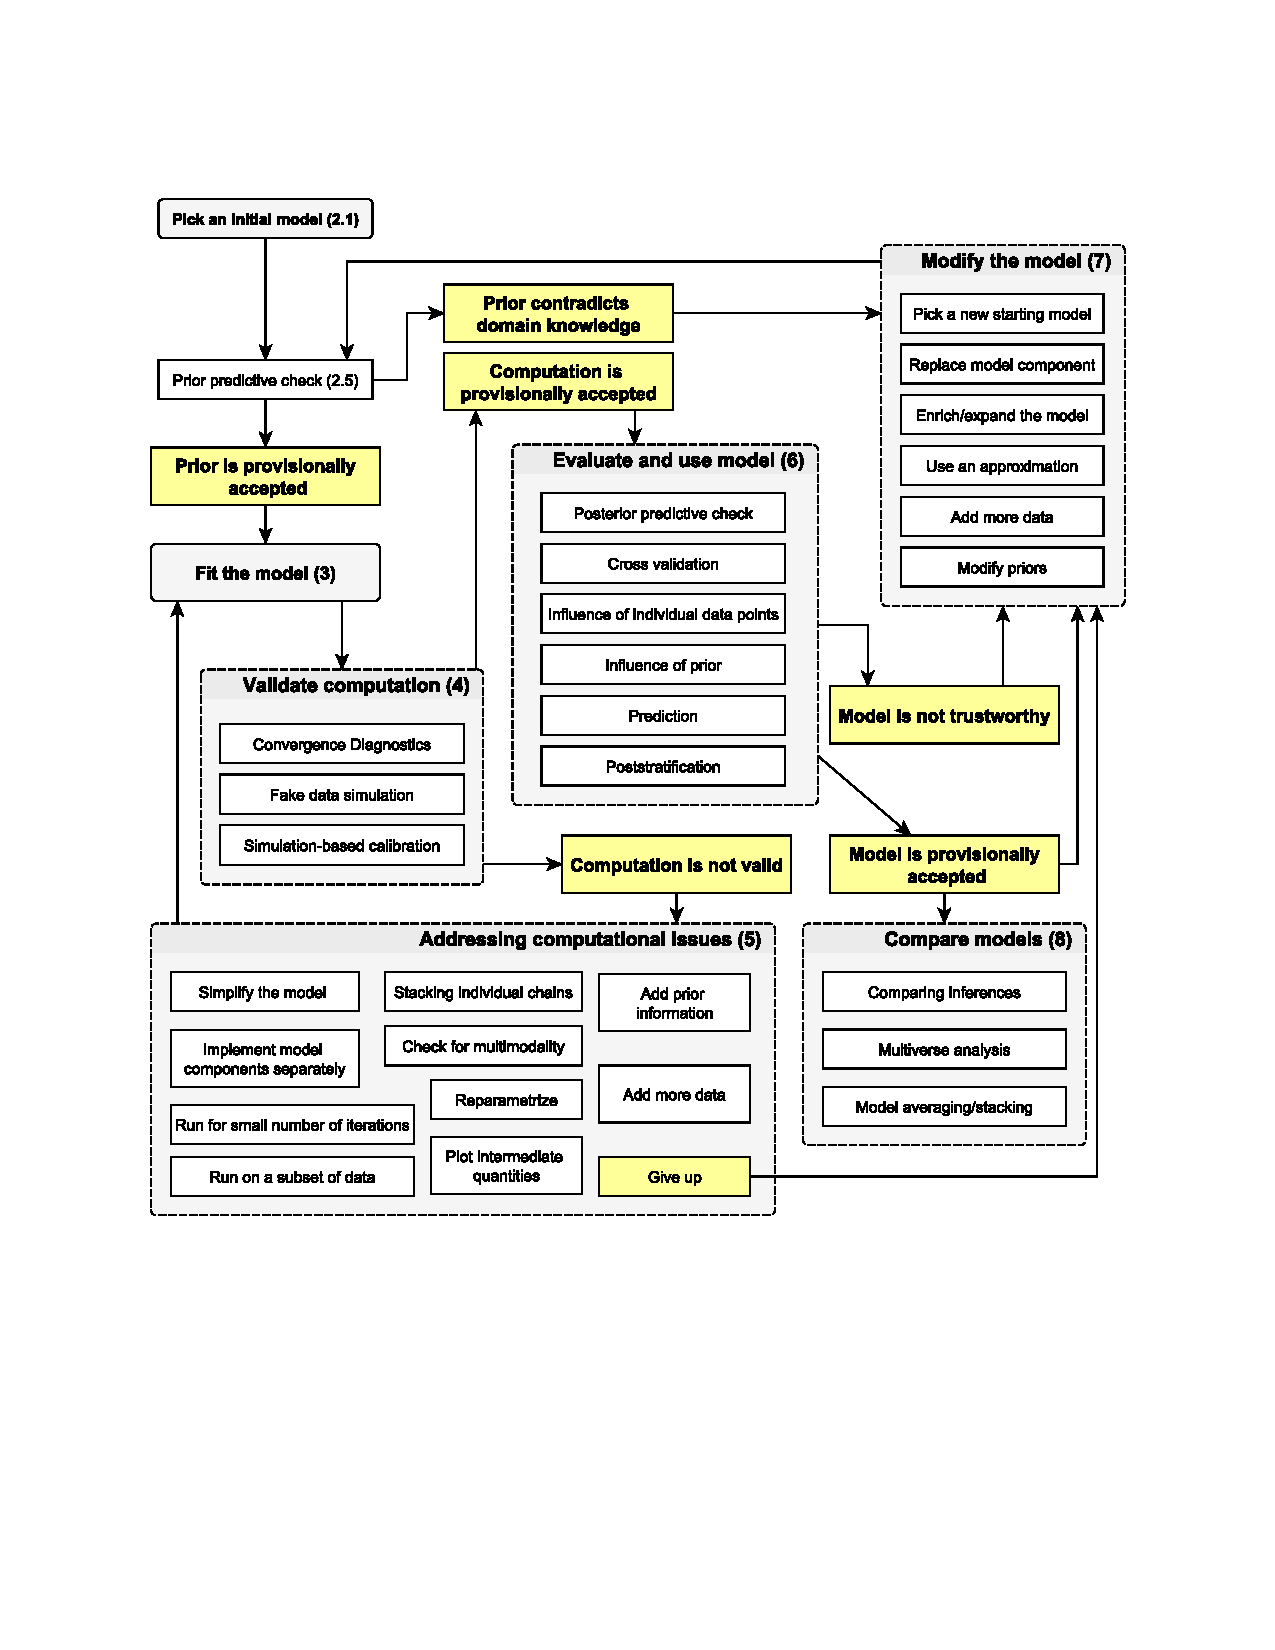
\includegraphics[height=0.7\textheight]{img/workflow-fig.pdf}
\end{center}
\begin{itemize}
\item where else might PPLs help?
\end{itemize}

\sld{Some more workflow issues}
\begin{itemize}
\item clamp/pin parameters to fixed values?
  \begin{subitemize}
    \item Stan requires moving the variable from the parameter to the
      data block
  \end{subitemize}
\item working with multiple (related) models?
  \begin{subitemize}
  \item model comparison
  \item model reparameterization
  \item model averaging/mixing/stacking
  \end{subitemize}
\item autogenerating parallel code?
  \begin{subitemize}
    \item Stan requires using parallel map functions in the program
  \end{subitemize}`
\end{itemize}

\sld{Naming and persistence is hard}
\begin{itemize}
\item how to \myemph{name and store multiple model variants}?
  \begin{subitemize}
    \item \texttt{uk-covid-icar}, \texttt{uk-covid-rw1}, \\
      \texttt{uk-covid-rw2}, \texttt{uk-covid-rw2-icar}, \\
      \texttt{uk-covid-rw2-bym2pc},  \texttt{uk-covid-rw2-bym2pc-no-socio},
      \textit{ad infinitum} $\ldots$
    \item plus multiple versions of the same model (over time)
  \end{subitemize}
\item how to \myemph{name and store output}?
\item how to work with \myemph{distributed teams}?
  \begin{subitemize}
  \item e.g., how to \myemph{share results} given that samples can be
    large?
  \item or that they run on clusters in pieces
  \end{subitemize}

\end{itemize}

\sld{Elephant in the room: Modularity}
\begin{itemize}
\item how to \myemph{modularize model components} like hierarchical
  priors or GP likelihoods
\item Stan lets users define \myemph{functions}
  \begin{subitemize}
  \item e.g., a random-walk or ICAR prior's density function
  \end{subitemize}
\item but they \myemph{can't cross block boundaries}, e.g., 
  data, parameter, model, generated quantities
\item how do other PPLs fare?
  \vfill
\item huge problem: \myemph{density is modular, behavior isn't}
\end{itemize}

\sld{References}
\begin{itemize}
\item \myemph{workflow paper}
  \begin{subitemize}
    \item Gelman, Vehtari, Simpson, Margossian, Carpenter, Yao, Kennedy,
    Gabry, Bürkner, Modrák. 2020. Bayesian workflow. \textit{arXiv}.
  \end{subitemize}
\item open-access \myemph{workflow book}
  \begin{subitemize}
  \item Above authors++. 2022? \textit{Bayesian Workflow}. Chapman \& Hall/CRC.
  \item GitHub repo: \\ {\small \url{https://github.com/jgabry/bayes-workflow-book}}
  \end{subitemize}
\end{itemize}
  

\end{document}

\vspace*{-6pt}
{\footnotesize 
\begin{verbatim}
\end{verbatim}
\vspace*{-8pt}}
